\documentclass[11pt,a4paper]{article}
\usepackage[margin=0mm]{geometry}
\usepackage[T1]{fontenc}
\usepackage{newtxtext}
\usepackage[scaled=.95]{sourcesanspro}
\usepackage{microtype}
\usepackage{xcolor}
\usepackage{graphicx}
\usepackage{array,tabularx,booktabs}
\usepackage[most]{tcolorbox}
\usepackage[absolute,overlay]{textpos}
\usepackage{amsmath}
\usepackage{ragged2e}
\usepackage{hyperref}
\hypersetup{hidelinks}

\pagestyle{empty}
\setlength{\parindent}{0pt}
\setlength{\parskip}{0pt}
\setlength{\tabcolsep}{1.15pt}
\renewcommand{\arraystretch}{1.02}
\textblockorigin{0mm}{0mm}

% =========================================================
% Colors
% =========================================================
\definecolor{Navy}{HTML}{064C70}
\definecolor{Navy2}{HTML}{0B5E87}
\definecolor{Sky}{HTML}{EFF6FA}
\definecolor{BlueSoft}{HTML}{F4F8FB}
\definecolor{GoldSoft}{HTML}{FCF7EA}
\definecolor{GraySoft}{HTML}{F5F6F7}
\definecolor{Ink}{HTML}{15202A}
\definecolor{Muted}{HTML}{53616C}
\definecolor{Line}{HTML}{B8C1C8}
\definecolor{Green}{HTML}{2A7C5A}

% =========================================================
% Typography
% =========================================================
\newcommand{\bodyfont}{\fontsize{11.2}{12.0}\selectfont}
\newcommand{\smallfont}{\fontsize{11.0}{11.7}\selectfont}
\newcommand{\captionfont}{\fontsize{9.8}{10.6}\selectfont}

\newcommand{\subhead}[1]{%
  {\sffamily\fontsize{11.8}{12.4}\selectfont\bfseries #1}%
}

\newcommand{\sectionfont}{%
  \sffamily\fontsize{14.0}{14.8}\selectfont\bfseries
}

\AtBeginDocument{\bodyfont\color{Ink}}

% =========================================================
% Main section box
% =========================================================
\newtcolorbox{sectionbox}[2][]{
  enhanced,
  width=\linewidth,
  colback=white,
  colframe=Line,
  boxrule=.45pt,
  arc=1.25mm,
  left=2.0mm,
  right=2.0mm,
  top=1.5mm,
  bottom=1.5mm,
  title=#2,
  colbacktitle=Navy,
  coltitle=white,
  fonttitle=\sectionfont,
  toptitle=1.15mm,
  bottomtitle=1.05mm,
  lefttitle=2.4mm,
  titlerule=0pt,
  #1
}

% =========================================================
% Soft card
% =========================================================
\newtcolorbox{softcard}[1]{
  enhanced,
  colback=#1,
  colframe=Line!70,
  boxrule=.35pt,
  arc=.9mm,
  left=1.3mm,
  right=1.3mm,
  top=1.0mm,
  bottom=1.0mm
}

% =========================================================
% Method card
% =========================================================
\newtcolorbox{methodcard}[1]{
  enhanced,
  height=22.5mm,
  valign=top,
  colback=#1,
  colframe=Line!78,
  boxrule=.35pt,
  arc=.9mm,
  left=1.45mm,
  right=1.45mm,
  top=1.15mm,
  bottom=1.0mm
}

\begin{document}
\thispagestyle{empty}

% =========================================================
% HEADER
% =========================================================
\begin{textblock*}{202mm}(4mm,4mm)

\begin{tcolorbox}[
  enhanced,
  height=23mm,
  valign=center,
  colback=white,
  colframe=Line,
  boxrule=.45pt,
  arc=1.4mm,
  left=2mm,
  right=2mm,
  top=.8mm,
  bottom=.8mm
]

\centering

{\sffamily
\fontsize{22.5}{22.8}\selectfont
\bfseries
OnePrompt-All: One Click to All Same-Concept Instances
}\par

\vspace{.45mm}

{\sffamily
\fontsize{12.5}{13.1}\selectfont
A training-free point-conditioned grounding framework for SAM 3
}\par

\vspace{.4mm}

{\sffamily\fontsize{10.8}{11.4}\selectfont
Wenzheng Huang
\quad $\cdot$ \quad
Shi Hu
\quad $\cdot$ \quad
Zihan Zhu
\quad $\cdot$ \quad
Haiyang Jin
\quad $\cdot$ \quad
Guangyao Shen
}\par

\vspace{.22mm}

{\sffamily\fontsize{10.3}{10.9}\selectfont\color{Muted}
School of AI and Advanced Computing
\hspace{2.2mm}\textbar\hspace{2.2mm}
\textbf{\color{Ink}Advisor: Kang Dang \quad $\cdot$ \quad Zhennong Chen}
}

\end{tcolorbox}

\end{textblock*}


% =========================================================
% PROBLEM
% =========================================================
\begin{textblock*}{51mm}(4mm,29mm)

\begin{sectionbox}[height=118mm]{Problem}

\subhead{Research question}\par

\vspace{.8mm}

{\fontsize{11.7}{12.3}\selectfont
Can one point trigger multi-instance segmentation in SAM 3?
}\par

\vspace{1.2mm}

\smallfont
OnePrompt-All asks whether a single point can trigger multi-instance grounding.
The click anchors SAM 3's pretrained visual representation and elicits
a concept-level response without category text or training.
\par

\vspace{1.0mm}

\subhead{Interaction paradigm}\par

\vspace{.45mm}

% PVS
\begin{tcolorbox}[
  enhanced,
  colback=GraySoft,
  colframe=Line!70,
  boxrule=.3pt,
  arc=.8mm,
  left=1.25mm,
  right=1.25mm,
  top=.65mm,
  bottom=.65mm
]
{\smallfont\textbf{PVS}}\par
{\smallfont Point $\rightarrow$ one instance}
\end{tcolorbox}

\vspace{.4mm}

% PCS
\begin{tcolorbox}[
  enhanced,
  colback=GoldSoft,
  colframe=Line!70,
  boxrule=.3pt,
  arc=.8mm,
  left=1.25mm,
  right=1.25mm,
  top=.65mm,
  bottom=.65mm
]
{\smallfont\textbf{PCS}}\par
{\smallfont Text $\rightarrow$ concept set}
\end{tcolorbox}

\vspace{.4mm}

% OnePrompt-All
\begin{tcolorbox}[
  enhanced,
  colback=Sky,
  colframe=Navy!42,
  boxrule=.45pt,
  arc=.8mm,
  left=1.25mm,
  right=1.25mm,
  top=.7mm,
  bottom=.7mm
]
{\smallfont\textbf{OnePrompt-All}}\par
{\smallfont Point $\rightarrow$ multi-instance response}
\end{tcolorbox}

\vfill

\end{sectionbox}

\end{textblock*}


% =========================================================
% METHOD
% =========================================================
\begin{textblock*}{148mm}(58mm,29mm)

\begin{sectionbox}[height=118mm]{Method}

\bodyfont
OnePrompt-All uses a positive click as a \textit{geometric condition} rather than
a category label. The click anchors the target in SAM 3's pretrained visual
representation, while learned object queries search the full image in parallel
for candidate instance masks. Lightweight post-processing then produces the
final instance set without additional training.
\par

\vspace{.65mm}

% ---------------------------------------------------------
% Method details: two balanced columns
% ---------------------------------------------------------
\begin{minipage}[t]{.488\linewidth}

\subhead{Point-conditioned grounding}\par
\vspace{.2mm}
\smallfont
The click supplies sparse spatial evidence about the intended object. SAM 3
injects this cue into the grounding pathway, so the detector is conditioned by
the selected location while still searching globally.

\vspace{.55mm}

\subhead{Candidate generation}\par
\vspace{.2mm}
\smallfont
Multiple object queries attend to conditioned image features in parallel.
Each produces a scored candidate mask, yielding valid instances,
weak fragments, and duplicate responses.
\end{minipage}
\hfill
\begin{minipage}[t]{.488\linewidth}

\subhead{Filtering and deduplication}\par
\vspace{.2mm}
\smallfont
Area filtering first removes trivial fragments using a class-agnostic size rule.
Mask NMS then suppresses highly overlapping predictions and keeps the stronger
candidate, yielding independent instance masks.

\vspace{.55mm}

\subhead{Optional DINOv2 ordering}\par
\vspace{.2mm}
\smallfont
Before NMS, DINOv2 may softly reorder candidates by similarity to the clicked
seed. It is auxiliary ranking rather than a hard semantic filter, so the core
pipeline remains training-free and category-agnostic.

\end{minipage}

\vspace{.65mm}

% ---------------------------------------------------------
% Fig. 1
% ---------------------------------------------------------
\begin{center}
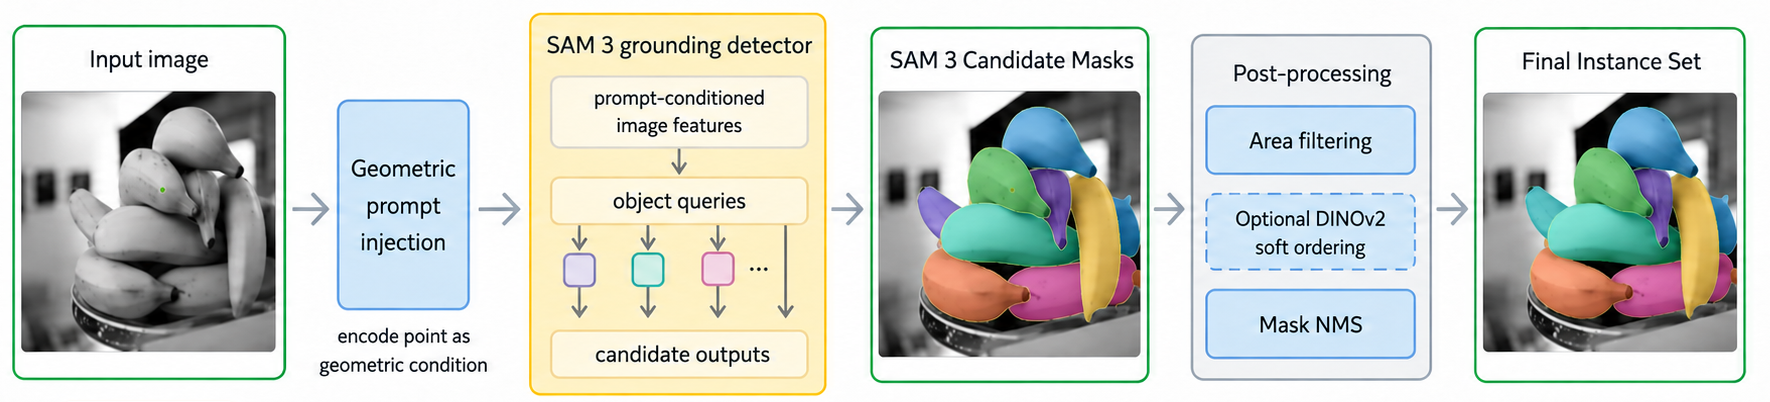
\includegraphics[
  width=.985\linewidth,
  height=34mm,
  keepaspectratio
]{figures/fig1_architecture2.jpg}
\end{center}

\end{sectionbox}
\end{textblock*}


% =========================================================
% RESULTS
% =========================================================
\begin{textblock*}{202mm}(4mm,150mm)

\begin{sectionbox}[height=108mm]{Results}

% ---------------------------------------------------------
% Compact result summary
% ---------------------------------------------------------
\begin{minipage}[t]{.475\linewidth}

\subhead{Evaluation}\par
\vspace{.15mm}
\smallfont
\textbf{Integrated OnePrompt-All Benchmark}: 2,220 images, 232 classes,
and 11,100 trials. Each run uses RGB + one positive click; ground truth is
used only for prompt sampling and scoring.

\end{minipage}
\hfill
\begin{minipage}[t]{.505\linewidth}

\subhead{Main findings}\par
\vspace{.15mm}
{\fontsize{10.6}{11.2}\selectfont
OnePrompt-All achieves \textbf{F1 0.667} and \textbf{mIoU 0.601},
with balanced precision (0.687) and recall (0.712) across the integrated
benchmark. Remaining errors are mainly caused by false candidates and
sensitivity to click location.
}
\end{minipage}

\vspace{.45mm}

% ---------------------------------------------------------
% Results table
% ---------------------------------------------------------
{\fontsize{9.6}{10.1}\selectfont
\setlength{\tabcolsep}{0.8pt}
\renewcommand{\arraystretch}{0.93}

\begin{tabularx}{\linewidth}{
  >{\raggedright\arraybackslash}p{24mm}
  >{\raggedright\arraybackslash}p{37mm}
  *{9}{>{\centering\arraybackslash}X}
}
\toprule
Method
& Benchmark
& Images
& Classes
& Runs
& F1
& F1 SD
& Prec.
& Recall
& mIoU
& IoU SD
\\

\midrule

OnePrompt-All
& Integrated Benchmark
& 2,220
& 232
& 11,100
& \textbf{0.667}
& 0.280
& 0.687
& 0.712
& \textbf{0.601}
& 0.279
\\

\bottomrule
\end{tabularx}
}

\vspace{.55mm}

% ---------------------------------------------------------
% Figures
% Fig. 3 is intentionally slightly larger than Fig. 2
% ---------------------------------------------------------
\makebox[\linewidth][c]{%

\begin{minipage}[t]{65mm}
\centering

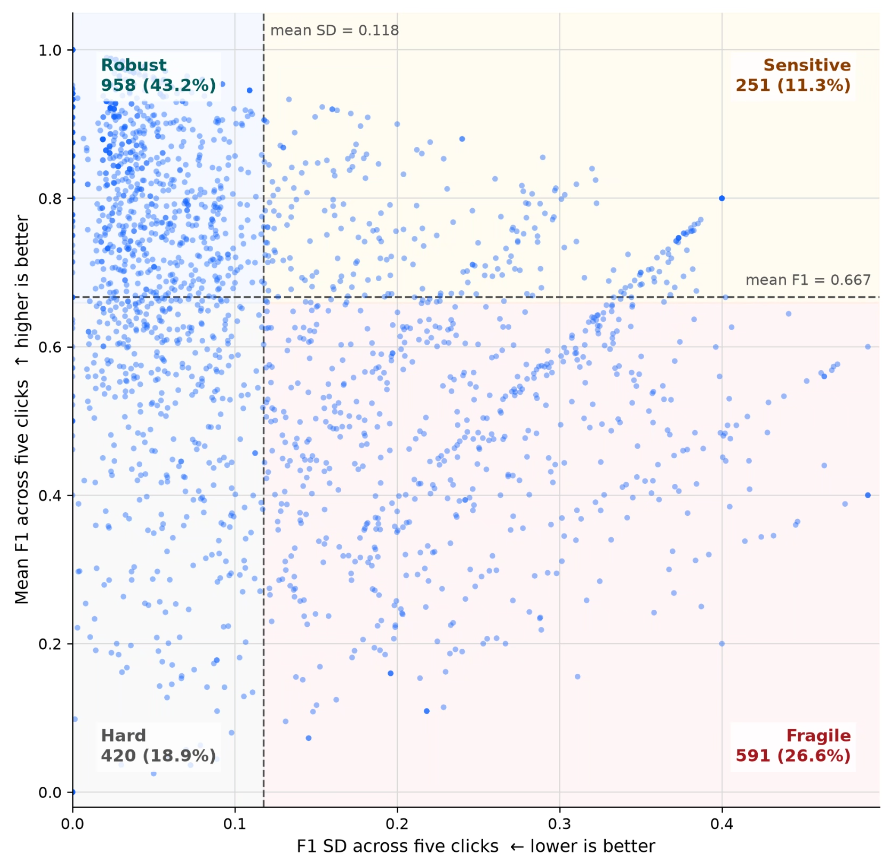
\includegraphics[
  height=52.5mm,
  keepaspectratio
]{figures/fig2_quadrant.png}

\vspace{.35mm}

\captionfont
\textit{
Fig. 2.
Accuracy vs. click robustness across 2,220 images;
dashed lines mark dataset means.
}

\end{minipage}

\hspace{3mm}

\begin{minipage}[t]{119mm}
\centering

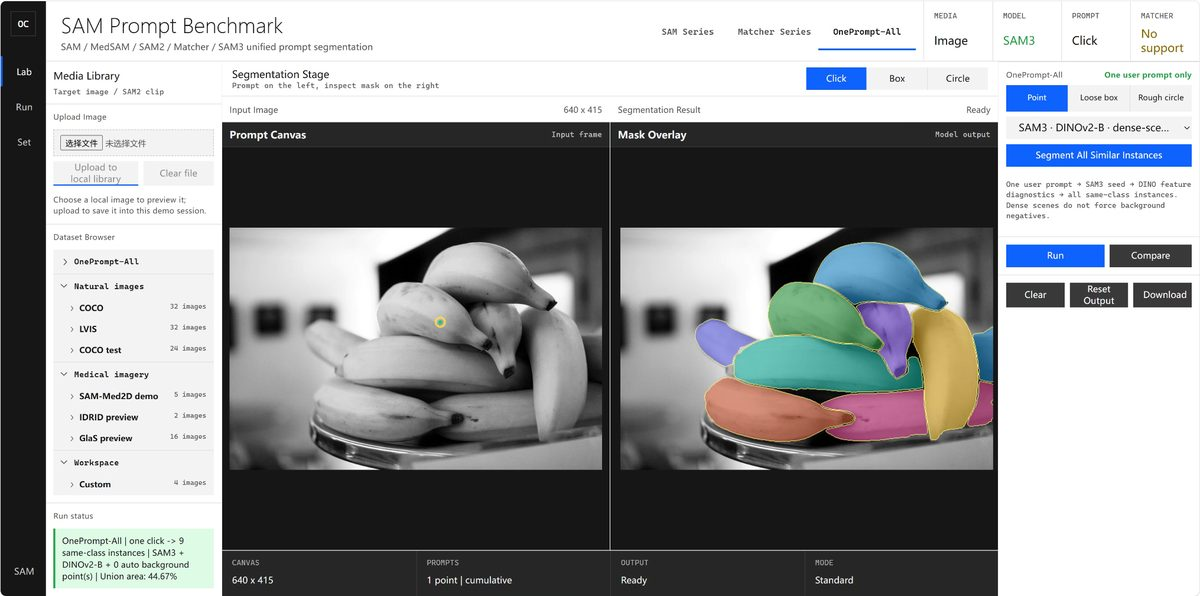
\includegraphics[
  height=54.5mm,
  keepaspectratio
]{figures/fig3_workbench.jpg}

\vspace{.35mm}

\captionfont
\textit{
Fig. 3.
Interactive workbench for prompting, model comparison, and mask inspection.
}

\end{minipage}%

}

\end{sectionbox}

\end{textblock*}


% =========================================================
% CONCLUSION
% =========================================================
\begin{textblock*}{202mm}(4mm,258.5mm)

\begin{sectionbox}[height=34mm]{Conclusion \& Discussion}

\noindent
\begin{minipage}[t]{.32\linewidth}
\subhead{Conclusion}\par
\vspace{.1mm}
{\fontsize{10.2}{10.8}\selectfont
A single point can trigger a multi-instance response in SAM 3, enabling
\textbf{training-free multi-instance segmentation}.
}
\end{minipage}%
\hfill%
\begin{minipage}[t]{.32\linewidth}
\subhead{Discussion}\par
\vspace{.1mm}
{\fontsize{10.2}{10.8}\selectfont
Global object queries recover related instances, while area filtering and
mask NMS suppress fragments and duplicates.
}
\end{minipage}%
\hfill%
\begin{minipage}[t]{.32\linewidth}
\subhead{Limitations}\par
\vspace{.1mm}
{\fontsize{10.2}{10.8}\selectfont
Performance still depends on click placement, occlusion, appearance variation,
and distractors; candidate calibration remains future work.
}
\end{minipage}

\end{sectionbox}

\end{textblock*}

\null

\end{document}